\graphicspath{{snoga/}}
\chapter{Supplementary Matarials for Chapter 4} %for Multi-objective Formulation of MSA for Phylogeny Inference
%\begin{subappendices}
%\renewcommand{\thesection}{\Alph{section}}%
%% or try \arabic{section}
%
%\section{Also you should know this}
%Really.
%\section{And I also came across this}
%But I need to put this in an appendix so that my paper is not too long.
%\end{subappendices}

%\section*{Appendix}

\section{Incomplete Lineage Sorting}%\index{Incomplete lineage sorting (ILS)}
Incomplete lineage sorting (ILS) refers to the failure of two gene lineages to coalesce at their speciation point. Also known as deep coalescence, this process is best understood under the coalescent model~\cite{degnan2006discordance, degnan2005gene}. This model explains evolutionary process by going backwards in time and connecting gene lineages to a common ancestor through a process of ``coalescence" of lineage pairs. In this model, each species is treated as a population of individuals, having a pair of alleles for each gene. The present day variants of a gene (known as alleles) are then traced back in time across successive generations by following the ancestral alleles in the previous generation from which this given alleles evolved. Eventually a point is reached where two alleles coalesce (i.e., they find a common ancestor). The multi-species coalescent (MSC) model is the extension of this general coalescent framework where multiple randomly mating populations corresponding to multiple species are present.
%, nei1987molecular, tajima1983evolutionary, takahata1989gene
\begin{figure}[!tb]
	\centering
	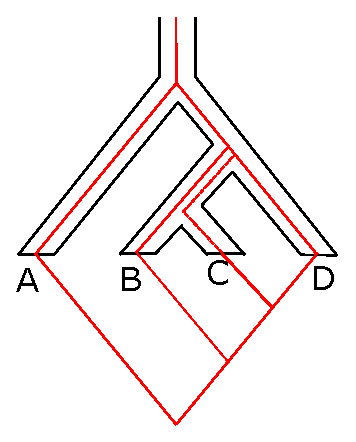
\includegraphics[width=0.33\textwidth]{Figure/ils.eps}
	\caption{Example of gene tree-species tree discordance due to incomplete lineage sorting. %Going back in time, the gene copies within species $B$ and $C$ first meet at their corresponding speciation point, but fail to coalesce. Both the lineages (dashed and solid black lines) exist on deeper ancestral branch. The gene from $C$ first coalesces with the gene from species $D$, and subsequently with the gene from $B$.
	}
	\label{fig:ils}
\end{figure}
Under the MSC model, ILS can be a source of gene tree discordance, as the common ancestry of gene copies at a single locus can extend deeper than speciation events. The larger the effective population size and the shorter the branch length of the evolutionary tree, the greater the chance of ILS or deep coalescence to occur~\cite{maddison1997gene}.

Figure~\ref{fig:ils} shows an example of discordance due to ILS. The gene copies within species $B$ and $C$ first meet at their corresponding speciation point as we go back in time. The speciation point is the most recent common ancestor of species $B$ and $C$. However, the gene copies fail to coalesce here. Both of these copies go further back in time, resulting in two gene lineages on deeper ancestral branch. The extra lineage is shown by the dashed red lines in Figure~\ref{fig:ils}. Then the gene from $C$ first coalesces with the gene from species $D$, and subsequently with the gene from $B$.